\begin{frame}{同期現象}
  \begin{itemize}
    \item 振動子が相互作用を通して振動のタイミングを揃える現象
    \begin{itemize}
      \item ホタルの発光
      \item メトロノーム
      \item ニューロンの発火、etc.
    \end{itemize}
  \begin{figure}
    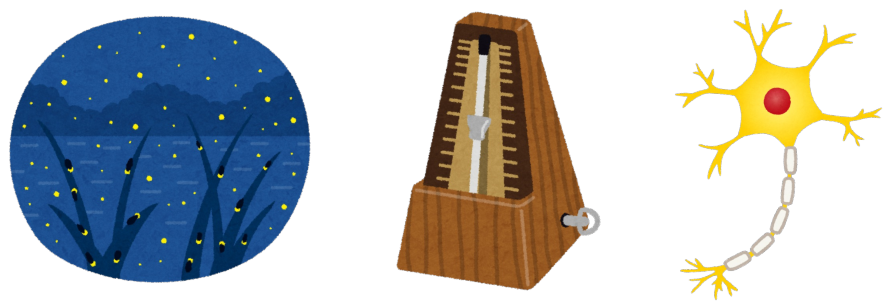
\includegraphics[height=0.2\textheight]{figs/sync_image.pdf}
  \end{figure}
%   \item ホイヘンスが振り子時計の振り子の運動が揃うことに気づいたことが最初
  \item 悪い側面も
  \begin{itemize}
    \item ミレニアム橋の崩壊
    \item てんかん発作
  \end{itemize}
  \begin{figure}
    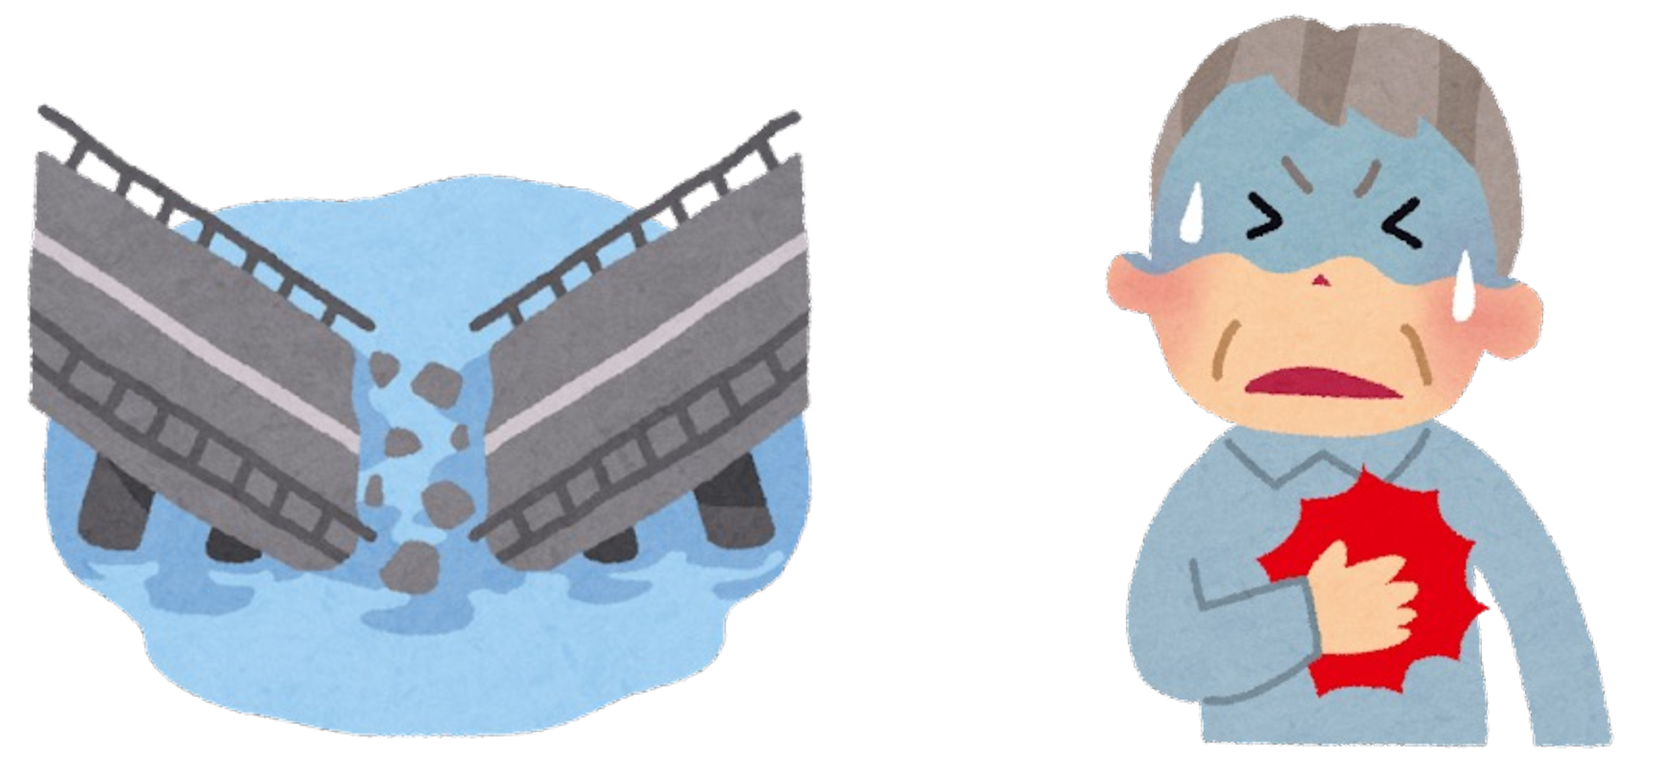
\includegraphics[height=0.2\textheight]{figs/sync_bad.pdf}
  \end{figure}
  \end{itemize}
\end{frame}

\begin{frame}{結合位相振動子系}
\begin{figure}
  \centering
  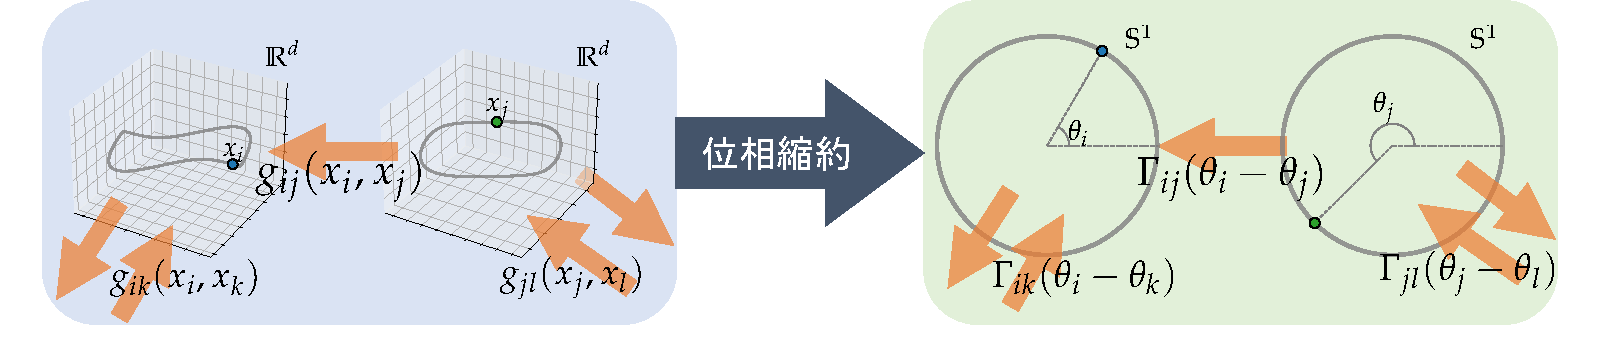
\includegraphics[width=\textwidth]{figs/phase_reduction.pdf}
\end{figure}
% \begin{block}{結合位相振動子系}
%   \centering
%   $\displaystyle \frac{\diff\theta_{i}}{\diff t}=\omega_{i}+\sum_{j=1}^{N}\Gamma_{ij}(\theta_{j}-\theta_{i})$
% \end{block}
\begin{align*}
  \frac{\diff\theta_{i}}{\diff t}=\redbox{\omega_{i}}{自然振動数}+\sum_{j=1}^{N}\redbox{\Gamma_{ij}(\theta_{i}-\theta_{j})}{結合関数}
\end{align*}
\begin{itemize}
  \item $\theta_{i}\in[0,2\pi)$: 各振動子の``位相''
  \item $\omega_{i}$: 各振動子が固有に持つ速度(自然振動数)
  \item $\Gamma_{ij}\colon\mathbb{S}^{1}\to\mathbb{R}$: 振動子間の\textbf{結合関数}
  \begin{itemize}
    \item 位相差$\theta_{j}-\theta_{i}$が入力
  \end{itemize}
\end{itemize}

\end{frame}

\begin{frame}{Questions}
\begin{itemize}
  \item \textbf{理論的側面} [Chapter 3, 4]
  \begin{figure}
    \centering
    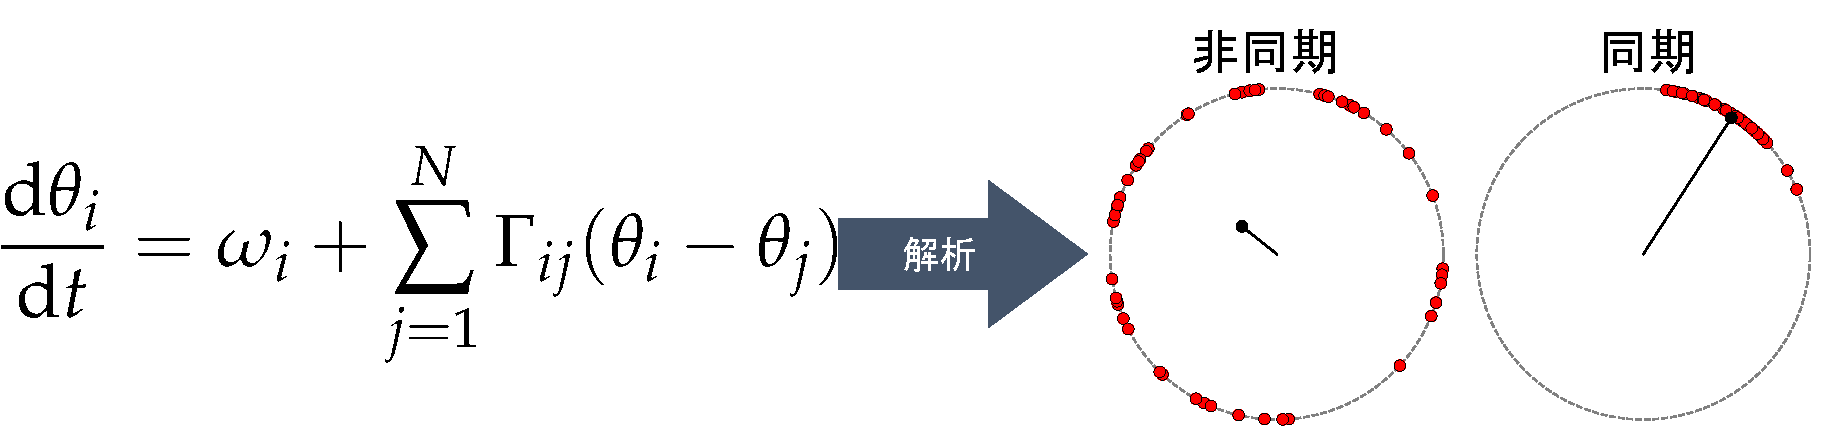
\includegraphics[width=0.7\textwidth]{figs/theory_ponchi.pdf}
  \end{figure}
  \begin{itemize}
    \item 非同期状態から同期状態への転移の振る舞いは?
    \item どのような条件のもとで同期しやすい/同期しにくいのか?
  \end{itemize}
  \item \textbf{実験的側面} [Chapter 5]
  \begin{figure}
    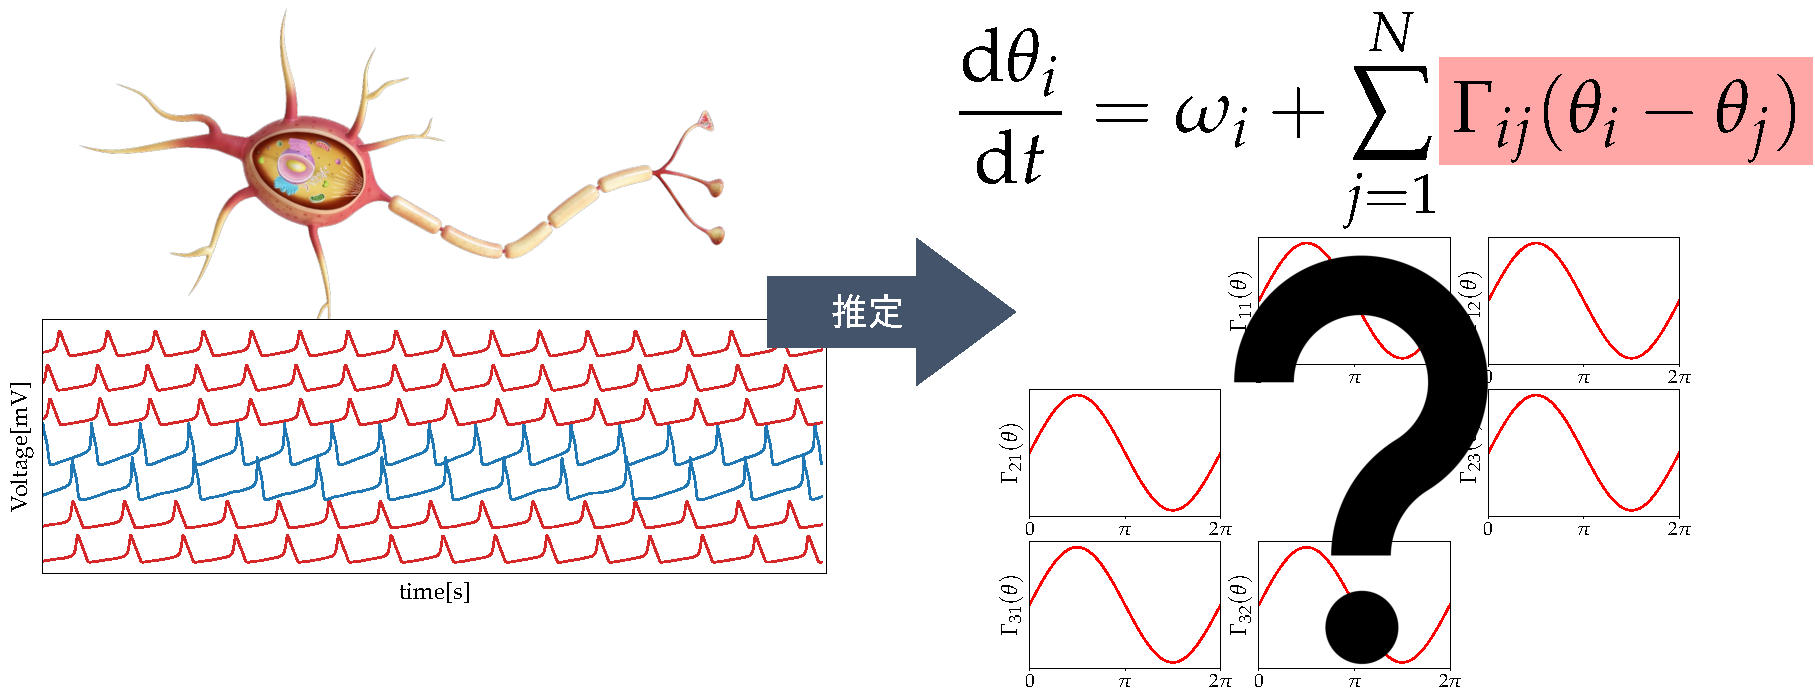
\includegraphics[width=0.7\textwidth]{figs/gp_coupling_ponchi.pdf}
  \end{figure}
  \begin{itemize}
    \item 与えられたデータからどのようにモデルを推定するか?
  \end{itemize}
\end{itemize}
\end{frame}

% \begin{frame}{Outline}
% \begin{figure}
%     \centering
%     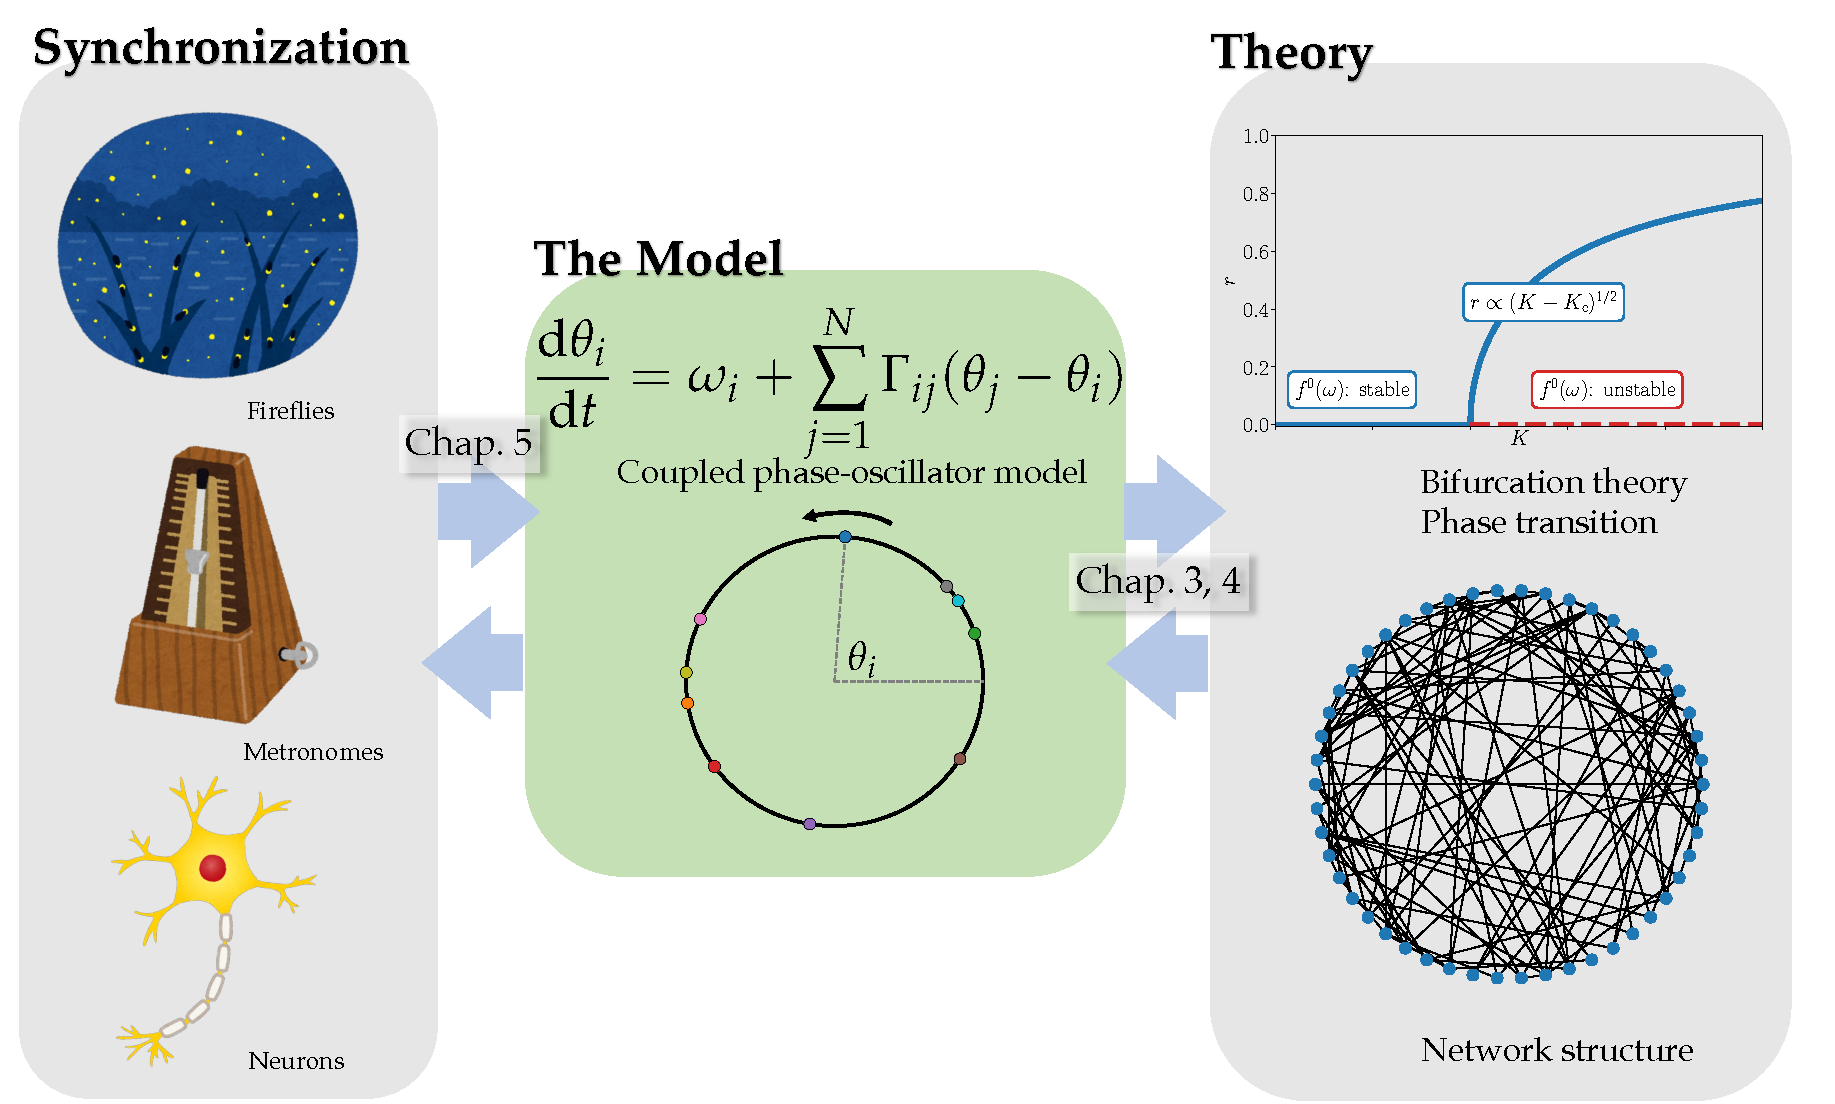
\includegraphics[width=\textwidth]{figs/phd_schematic.pdf}
% \end{figure}
% \end{frame}

\begin{frame}{博士論文の構成}
\begin{itemize}
  \item \lightgray{\textbf{Chapter 1}: イントロダクション}
  \item \lightgray{\textbf{Chapter 2}: 結合位相振動子系のレビュー}
  \item \textbf{Chapter 3}: Critical exponents in coupled phase-oscillator models on small-world networks
  \begin{itemize}
    \item Published in Physical Review E (2020)
  \end{itemize}
  \item \textbf{Chapter 4}: The lower bound of the network connectivity guaranteeing in-phase synchronization
  \begin{itemize}
    \item Published in Chaos (2021)
  \end{itemize}
  \item \textbf{Chapter 5}: Gaussian process regression approach to estimating phase dynamics from rhythmic data
  \begin{itemize}
    \item In preparation ...
  \end{itemize}
  \item \lightgray{\textbf{Chapter 6}: まとめ}
\end{itemize}
\end{frame}